%This work is licensed under the Creative Commons License Attribution 4.0 International (CC-BY 4.0) 
%https://creativecommons.org/licenses/by/4.0/legalcode 
\documentclass[rgb]{standalone}
\usepackage{tkz-euclide}
\usetikzlibrary{matrix}
\begin{document}
	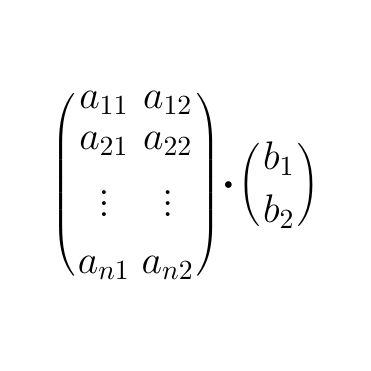
\begin{tikzpicture}[scale=0.5, font=\Large]
		\draw[draw=none] (-2.75,-4) -- (-2.75,4) -- (5.25,4) -- (5.25,-4) -- cycle;
		\matrix [matrix of math nodes,column sep=-0.25em,outer sep=-7,left delimiter=(,right delimiter=)](A){ 
			a_{11} & a_{12}   \\
			a_{21} & a_{22}   \\
			\vdots & \vdots\vphantom{a_{22}} \\
			a_{n1} & a_{n2}\vphantom{a^{22}}   \\
		};
		\matrix [xshift=-0.1cm,right =of A,matrix of math nodes,column sep=-0.25em,outer sep=-7,left delimiter=(,right delimiter=)](B){ 
			b_{1}    \\
			b_{2}    \\
		};
		\tkzLabelPoint[anchor=center](2.35,0){\tiny$\bullet$}
	\end{tikzpicture}
\end{document}